% $Author: oscar $
% $Date: 2009-09-15 16:53:48 +0200 (Tue, 15 Sep 2009) $
% $Revision: 29111 $
%=================================================================
\ifx\wholebook\relax\else
% --------------------------------------------
% Lulu:
	\documentclass[a4paper,10pt,twoside]{book}
	\usepackage[
		papersize={6.13in,9.21in},
		hmargin={.815in,.815in},
		vmargin={.98in,.98in},
		ignoreheadfoot
	]{geometry}
	\usepackage[hangul]{kotex}
	% $Author: oscar $
% $Date: 2009-09-13 20:58:29 +0200 (Sun, 13 Sep 2009) $
% $Revision: 29070 $
%=============================================================
% NB: documentclass must be set in main document.
% Allows book to be generated in multiple formats.
%=============================================================
%:Packages
\usepackage[T1]{fontenc}  %%%%%really important to get the code directly in the text!
\usepackage{palatino}
\usepackage{ifthen}
\usepackage{graphicx}
\graphicspath{{figures/}}
\usepackage{xspace}
\usepackage{makeidx}
\usepackage{isodateo} % enable \isodate
\usepackage{amssymb,textcomp}
%=============================================================
%:More packages
%\usepackage[english]{babel}
%\usepackage{lmodern}
%\usepackage[scaled=0.85]{helvet}
%\usepackage{microtype}
%\usepackage{theorem}
%\usepackage{float}
%\usepackage{longtable}
%\usepackage[nottoc]{tocbibind}
%\usepackage{multicol}
%\usepackage{booktabs}	% book-style tables
%\usepackage{topcapt}	% enables \topcaption
%\usepackage{multirow}
%\usepackage{tabularx}
%\usepackage{alltt}
\usepackage[usenames,dvipsnames]{color}
%\usepackage[hang]{subfigure}\makeatletter\def\p@subfigure{\thefigure\,}\makeatother
%\usepackage{rotating}
%\usepackage{enumitem}	% apb: allows more control over tags in enumerations
%\usepackage{verbatim}     % for comment environment
%\usepackage{varioref}	% for page references that work
%\usepackage{needspace}
%\usepackage[newparttoc]{titlesec}
%\usepackage{titletoc}
%\usepackage{wrapfig}
\usepackage[
	colorlinks=true,
	linkcolor=black,
	urlcolor=black,
	citecolor=black
]{hyperref}   % should come last
%=============================================================
%:URL style
\makeatletter
\def\url@leostyle{%
  \@ifundefined{selectfont}{\def\UrlFont{\sf}}{\def\UrlFont{\sffamily}}}
\makeatother
\urlstyle{leo}
%=============================================================
%:Booleans
\newboolean{lulu}
\setboolean{lulu}{false}
\newcommand{\ifluluelse}[2]{\ifthenelse{\boolean{lulu}}{#1}{#2}}
%=============================================================
%:Editorial comment macros
\newcommand{\nnbb}[2]{
  \fbox{\bfseries\sffamily\scriptsize#1}
  {\sf\small$\blacktriangleright$\textit{#2}$\blacktriangleleft$}
}
\newcommand{\on}[1]{\nnbb{Oscar}{#1}}
\newcommand{\here}{\nnbb{CONTINUE}{HERE}}
%=============================================================
%:Abbreviation macros
\newcommand{\ie}{\emph{i.e.},\xspace}
\newcommand{\eg}{\emph{e.g.},\xspace}
\newcommand{\etc}{\emph{etc.}\xspace}
\newcommand{\etal}{\emph{et al.}\xspace}
\newcommand{\straightquote}{"}
\newcommand{\sba}{\url{SquareBracketAssociates.org}\xspace}
%=============================================================
%:Patterns
% \newcommand{\pattern}[2]{\newpage\section{{\sf #1}}\label{pat:#2}}
% \newcommand{\pattern}[2]{\newpage\index{#1 (Pattern)}\section{#1}\label{pat:#2}}
\newcommand{\pattern}[2]{\cleardoublepage\index{#1 (패턴)}\section{#1}\label{pat:#2}}
\newcommand{\thumbnail}[2]{\index{#1 (패턴)}\subsection{#1}\label{pat:#2}}
\newcommand{\thumblang}[2]{\index{#1 (패턴 랭귀지)}\subsection{#1}\label{pat:#2}}
\newcommand{\variant}[1]{{\emph{#1}}\xspace}
% \newcommand{\problem}[1]{\subsection*{Problem}\emph{#1}}
\newcommand{\intent}[1]{\paragraph{의도}\emph{#1}}
\newcommand{\problem}[1]{\paragraph{문제}\emph{#1}}
\newcommand{\solution}[1]{\paragraph{해결}\emph{#1}}
\newcommand{\discussion}[0]{\paragraph{토론}}
\newcommand{\cmd}[1]{{\tt #1}\xspace}
%=============================================================
%:Environments
\newenvironment{bulletlist}{\begin{itemize}\setlength{\itemsep}{0ex}}
{\end{itemize}}
%=============================================================
%:Cross reference macros
\newcommand{\chalabel}[1]{\label{cha:#1}}
\newcommand{\seclabel}[1]{\label{sec:#1}}
\newcommand{\figlabel}[1]{\label{fig:#1}}
\newcommand{\tablabel}[1]{\label{tab:#1}}
\newcommand{\rulelabel}[1]{\label{rule:#1}}
\newcommand{\eglabel}[1]{\label{eg:#1}}
\newcommand{\scrlabel}[1]{\label{scr:#1}}
\newcommand{\mthlabel}[1]{\label{mth:#1}}
\newcommand{\clslabel}[1]{\label{cls:#1}}
\newcommand{\faqlabel}[1]{\label{faq:#1}}
%\newcommand{\charef}[1]{Chapter~\ref{cha:#1}\xspace}
%\newcommand{\secref}[1]{Section~\ref{sec:#1}\xspace}
\newcommand{\figref}[1]{Figure~\ref{fig:#1}\xspace}
% \newcommand{\patpgref}[2]{\hyperref[pat:#2]{\sf #1} [p.~\pageref{pat:#2}]\xspace}
\newcommand{\patpgref}[2]{\index{#1 (Pattern)}\hyperref[pat:#2]{#1} [p.~\pageref{pat:#2}]\xspace}
\newcommand{\patlangpgref}[2]{\index{#1 (Pattern language)}\hyperref[pat:#2]{#1} [p.~\pageref{pat:#2}]\xspace}
% \newcommand{\patref}[2]{\hyperref[pat:#2]{\sf #1}\xspace}
\newcommand{\patref}[2]{\index{#1 (Pattern)}\hyperref[pat:#2]{#1}\xspace}
\newcommand{\patlangref}[2]{\index{#1 (Pattern language)}\hyperref[pat:#2]{#1}\xspace}
% \newcommand{\charef}[2]{\hyperref[cha:#2]{\underline{\sf #1}}\xspace}
% \newcommand{\charef}[2]{\hyperref[cha:#2]{\sf #1}\xspace}
\newcommand{\charef}[2]{\index{#1 (Pattern cluster)}\hyperref[cha:#2]{#1}\xspace}
% \newcommand{\chapgref}[2]{\hyperref[cha:#2]{\sf #1} [p.~\pageref{cha:#2}]\xspace}
\newcommand{\chapgref}[2]{\index{#1 (Pattern cluster)}\hyperref[cha:#2]{#1} [p.~\pageref{cha:#2}]\xspace}
%\newcommand{\Figref}[1]{Figure~\ref{fig:#1}\xspace}
%\newcommand{\appref}[1]{Appendix~\ref{app:#1}\xspace}
%\newcommand{\tabref}[1]{Table~\ref{tab:#1}\xspace}
%\newcommand{\ruleref}[1]{\ref{rule:#1}\xspace}
%\newcommand{\egref}[1]{example~\ref{eg:#1}\xspace}
%\newcommand{\Egref}[1]{Example~\ref{eg:#1}\xspace}
%\newcommand{\scrref}[1]{script~\ref{scr:#1}\xspace}
%\newcommand{\Scrref}[1]{Script~\ref{scr:#1}\xspace}
%\newcommand{\tscrref}[1]{the script~\ref{scr:#1}\xspace}
%\newcommand{\Tscrref}[1]{The script~\ref{scr:#1}\xspace}
%\newcommand{\mthref}[1]{method~\ref{mth:#1}\xspace}
%\newcommand{\mthsref}[1]{methods~\ref{mth:#1}\xspace}
%\newcommand{\Mthref}[1]{Method~\ref{mth:#1}\xspace}
%\newcommand{\tmthref}[1]{the method~\ref{mth:#1}\xspace}
%\newcommand{\Tmthref}[1]{The method~\ref{mth:#1}\xspace}
%\newcommand{\clsref}[1]{class~\ref{cls:#1}\xspace}
%\newcommand{\tclsref}[1]{the class~\ref{cls:#1}\xspace}
%\newcommand{\Tclsref}[1]{The class~\ref{cls:#1}\xspace}
%=============================================================
%:Page Layout
\setlength{\headsep}{1cm}
%=============================================================
%:Menu item macro
%\definecolor{lightgray}{gray}{0.89}
%\newcommand{\menu}[1]{{%
%	\setlength{\fboxsep}{0pt}%
%	\colorbox{lightgray}{{{\upshape\sffamily\strut \,#1\,}}}}}
%\newcommand{\go}{\,$\triangleright$\,}
%\newcommand{\short}[1]{\mbox{{\sc cmd}\hspace{0.08em}--\hspace{0.09em}#1}\xspace}
%\newcommand{\button}[1]{{%
%	\setlength{\fboxsep}{0pt}%
%	\fbox{{\upshape\sffamily\strut \,#1\,}}}}
%\newcommand{\toolsflap}{\textit{Tools} flap\xspace}
%=============================================================
%:Section depth
%\setcounter{secnumdepth}{2}
%
%\DeclareGraphicsExtensions{.pdf, .jpg, .png}
%=============================================================
%:PDF setup
\hypersetup{
   pdftitle={Object-Oriented Reengineering Patterns},
   pdfauthor={Serge Demeyer, St\'ephane Ducasse, Oscar Nierstrasz},
   pdfkeywords={Reengineering, Object-Oriented Programming, Patterns},
   pdfsubject={Computer Science}
}
%=============================================================
%:Page layout and appearance
%\renewcommand{\chaptermark}[1]{\markboth{#1}{}}
%\renewcommand{\sectionmark}[1]{\markright{\thesection\ #1}}
%\renewpagestyle{plain}[\small\itshape]{%
%	\setheadrule{0pt}%
%	\sethead[][][]{}{}{}%
%	\setfoot[][][]{}{}{}}
%\renewpagestyle{headings}[\small\itshape]{%
%	\setheadrule{0pt}%
%	\setmarks{chapter}{section}%
%	\sethead[\thepage][][\chaptertitle]{\sectiontitle}{}{\thepage}%
%	\setfoot[][][]{}{}{}}
%=============================================================
%:Title section setup and TOC numbering depth
%\setcounter{secnumdepth}{1}
%\setcounter{tocdepth}{1}
%\titleformat{\part}[display]{\centering}{\huge\partname\ \thepart}{1em}{\Huge\textbf}[]
%\titleformat{\chapter}[display]{}{\huge\chaptertitlename\ \thechapter}{1em}{\Huge\raggedright\textbf}[]
%\titlecontents{part}[3pc]{%
%		\pagebreak[2]\addvspace{1em plus.4em minus.2em}%
%		\leavevmode\large\bfseries}
%	{\contentslabel{3pc}}{\hspace*{-3pc}}
%	{}[\nopagebreak]
%\titlecontents{chapter}[3pc]{%
%		\pagebreak[0]\addvspace{1em plus.2em minus.2em}%
%		\leavevmode\bfseries}
%	{\contentslabel{3pc}}{}
%	{\hfill\contentspage}[\nopagebreak]
%\dottedcontents{section}[3pc]{}{3pc}{1pc}
%\dottedcontents{subsection}[3pc]{}{0pc}{1pc}
%\let\origdoublepage\cleardoublepage
%\newcommand{\clearemptydoublepage}{%
%  \clearpage
%  {\pagestyle{empty}\origdoublepage}}
%\let\cleardoublepage\clearemptydoublepage % see http://www.tex.ac.uk/cgi-bin/texfaq2html?label=patch
%=============================================================
%:Listings package configuration
\newcommand{\caret}{\makebox{\raisebox{0.4ex}{\footnotesize{$\wedge$}}}}
% \newcommand{\escape}{{\sf \textbackslash}}
\definecolor{source}{gray}{0.95}
\usepackage{listings}
\lstdefinelanguage{Smalltalk}{
  morestring=[d]',
% Adapt this to other languages!
%  morecomment=[s]{"}{"},
  alsoletter={\#:},
  %escapechar={!},
  literate=
    {BANG}{!}1
%    {UNDERSCORE}{\_}1
    {\\st}{Smalltalk}9 % convenience -- in case \st occurs in code
    % {'}{{\textquotesingle}}1 % replaced by upquote=true in \lstset
%    {_}{{$\leftarrow$}}1
    {>>>}{{\sep}}1
    {^}{{$\uparrow$}}1
    {~}{{$\sim$}}1
    {-}{{\sf -\hspace{-0.13em}-}}1  % the goal is to make - the same width as +
    {+}{\raisebox{0.08ex}{+}}1		% and to raise + off the baseline to match -
    {-->}{{\quad$\longrightarrow$\quad}}3
	, % Don't forget the comma at the end!
  tabsize=4
}[keywords,comments,strings]

\lstset{language=Smalltalk,
	basicstyle=\sffamily,
	keywordstyle=\color{black}\bfseries,
	% stringstyle=\ttfamily, % Ugly! do we really want this? -- on
	mathescape=true,
	showstringspaces=false,
	keepspaces=true,
	breaklines=true,
	breakautoindent=true,
	backgroundcolor=\color{source},
	lineskip={-1pt}, % Ugly hack
	upquote=true, % straight quote; requires textcomp package
	columns=fullflexible} % no fixed width fonts
% \newcommand{\ct}{\lstinline[mathescape=false,basicstyle={\sffamily\upshape}]}
\newcommand{\ct}{\lstinline[mathescape=false,backgroundcolor=\color{white},basicstyle={\sffamily\upshape}]}
\newcommand{\lct}[1]{{\textsf{\textup{#1}}}}
%\newcommand{\scat}[1]{\emph{\textsf{#1}}\xspace}
%\newcommand{\prot}[1]{\emph{\textsf{#1}}\xspace}
% NB: No argument!
\lstnewenvironment{code}[0]{%
	\lstset{%
		% frame=lines,
		frame=single,
		framerule=0pt,
		mathescape=false
	}
}{}
%\def\ignoredollar#1{}
%=============================================================
%:Reserving space
%\newcommand{\needlines}[1]{\Needspace{#1\baselineskip}}
%=============================================================
%:Indexing macros
% Macros ending with "ind" generate text as well as an index entry
% Macros ending with "index" *only* generate an index entry
\newcommand{\ind}[1]{\index{#1}#1\xspace} % plain text
\newcommand{\subind}[2]{\index{#1!#2}#2\xspace} % show #2, subindex under #1
\newcommand{\emphind}[1]{\index{#1}\emph{#1}\xspace} % emph #1
\newcommand{\emphsubind}[2]{\index{#1!#2}\emph{#2}\xspace} % show emph #2, subindex under #1
\newcommand{\patind}[1]{\index{#1@#1 (pattern)}\ct{#1}\xspace} % pattern
\newcommand{\seeindex}[2]{\index{#1|see{#2}}} % #1, see #2
%\newcommand{\boldidx}[1]{{\bf #1}} % breaks hyperlink
%\newcommand{\indmain}[1]{\index{#1}#1\xspace} 
%\newcommand{\emphsubindmain}[2]{\index{#1!#2}\emph{#2}\xspace} % subindex, main entry
%\newcommand{\subindmain}[2]{\index{#1!#2}#2\xspace} % subindex, main entry
%\newcommand{\clsindmain}[1]{\index{#1!\#@(class)}\ct{#1}\xspace} % class main
%\newcommand{\indexmain}[1]{\index{#1}} 
%=============================================================
\parskip 1ex
%=============================================================

	\pagestyle{headings}
	\setboolean{lulu}{true}
% --------------------------------------------
% A4:
%	\documentclass[a4paper,11pt,twoside]{book}
%	% $Author: oscar $
% $Date: 2009-09-13 20:58:29 +0200 (Sun, 13 Sep 2009) $
% $Revision: 29070 $
%=============================================================
% NB: documentclass must be set in main document.
% Allows book to be generated in multiple formats.
%=============================================================
%:Packages
\usepackage[T1]{fontenc}  %%%%%really important to get the code directly in the text!
\usepackage{palatino}
\usepackage{ifthen}
\usepackage{graphicx}
\graphicspath{{figures/}}
\usepackage{xspace}
\usepackage{makeidx}
\usepackage{isodateo} % enable \isodate
\usepackage{amssymb,textcomp}
%=============================================================
%:More packages
%\usepackage[english]{babel}
%\usepackage{lmodern}
%\usepackage[scaled=0.85]{helvet}
%\usepackage{microtype}
%\usepackage{theorem}
%\usepackage{float}
%\usepackage{longtable}
%\usepackage[nottoc]{tocbibind}
%\usepackage{multicol}
%\usepackage{booktabs}	% book-style tables
%\usepackage{topcapt}	% enables \topcaption
%\usepackage{multirow}
%\usepackage{tabularx}
%\usepackage{alltt}
\usepackage[usenames,dvipsnames]{color}
%\usepackage[hang]{subfigure}\makeatletter\def\p@subfigure{\thefigure\,}\makeatother
%\usepackage{rotating}
%\usepackage{enumitem}	% apb: allows more control over tags in enumerations
%\usepackage{verbatim}     % for comment environment
%\usepackage{varioref}	% for page references that work
%\usepackage{needspace}
%\usepackage[newparttoc]{titlesec}
%\usepackage{titletoc}
%\usepackage{wrapfig}
\usepackage[
	colorlinks=true,
	linkcolor=black,
	urlcolor=black,
	citecolor=black
]{hyperref}   % should come last
%=============================================================
%:URL style
\makeatletter
\def\url@leostyle{%
  \@ifundefined{selectfont}{\def\UrlFont{\sf}}{\def\UrlFont{\sffamily}}}
\makeatother
\urlstyle{leo}
%=============================================================
%:Booleans
\newboolean{lulu}
\setboolean{lulu}{false}
\newcommand{\ifluluelse}[2]{\ifthenelse{\boolean{lulu}}{#1}{#2}}
%=============================================================
%:Editorial comment macros
\newcommand{\nnbb}[2]{
  \fbox{\bfseries\sffamily\scriptsize#1}
  {\sf\small$\blacktriangleright$\textit{#2}$\blacktriangleleft$}
}
\newcommand{\on}[1]{\nnbb{Oscar}{#1}}
\newcommand{\here}{\nnbb{CONTINUE}{HERE}}
%=============================================================
%:Abbreviation macros
\newcommand{\ie}{\emph{i.e.},\xspace}
\newcommand{\eg}{\emph{e.g.},\xspace}
\newcommand{\etc}{\emph{etc.}\xspace}
\newcommand{\etal}{\emph{et al.}\xspace}
\newcommand{\straightquote}{"}
\newcommand{\sba}{\url{SquareBracketAssociates.org}\xspace}
%=============================================================
%:Patterns
% \newcommand{\pattern}[2]{\newpage\section{{\sf #1}}\label{pat:#2}}
% \newcommand{\pattern}[2]{\newpage\index{#1 (Pattern)}\section{#1}\label{pat:#2}}
\newcommand{\pattern}[2]{\cleardoublepage\index{#1 (패턴)}\section{#1}\label{pat:#2}}
\newcommand{\thumbnail}[2]{\index{#1 (패턴)}\subsection{#1}\label{pat:#2}}
\newcommand{\thumblang}[2]{\index{#1 (패턴 랭귀지)}\subsection{#1}\label{pat:#2}}
\newcommand{\variant}[1]{{\emph{#1}}\xspace}
% \newcommand{\problem}[1]{\subsection*{Problem}\emph{#1}}
\newcommand{\intent}[1]{\paragraph{의도}\emph{#1}}
\newcommand{\problem}[1]{\paragraph{문제}\emph{#1}}
\newcommand{\solution}[1]{\paragraph{해결}\emph{#1}}
\newcommand{\discussion}[0]{\paragraph{토론}}
\newcommand{\cmd}[1]{{\tt #1}\xspace}
%=============================================================
%:Environments
\newenvironment{bulletlist}{\begin{itemize}\setlength{\itemsep}{0ex}}
{\end{itemize}}
%=============================================================
%:Cross reference macros
\newcommand{\chalabel}[1]{\label{cha:#1}}
\newcommand{\seclabel}[1]{\label{sec:#1}}
\newcommand{\figlabel}[1]{\label{fig:#1}}
\newcommand{\tablabel}[1]{\label{tab:#1}}
\newcommand{\rulelabel}[1]{\label{rule:#1}}
\newcommand{\eglabel}[1]{\label{eg:#1}}
\newcommand{\scrlabel}[1]{\label{scr:#1}}
\newcommand{\mthlabel}[1]{\label{mth:#1}}
\newcommand{\clslabel}[1]{\label{cls:#1}}
\newcommand{\faqlabel}[1]{\label{faq:#1}}
%\newcommand{\charef}[1]{Chapter~\ref{cha:#1}\xspace}
%\newcommand{\secref}[1]{Section~\ref{sec:#1}\xspace}
\newcommand{\figref}[1]{Figure~\ref{fig:#1}\xspace}
% \newcommand{\patpgref}[2]{\hyperref[pat:#2]{\sf #1} [p.~\pageref{pat:#2}]\xspace}
\newcommand{\patpgref}[2]{\index{#1 (Pattern)}\hyperref[pat:#2]{#1} [p.~\pageref{pat:#2}]\xspace}
\newcommand{\patlangpgref}[2]{\index{#1 (Pattern language)}\hyperref[pat:#2]{#1} [p.~\pageref{pat:#2}]\xspace}
% \newcommand{\patref}[2]{\hyperref[pat:#2]{\sf #1}\xspace}
\newcommand{\patref}[2]{\index{#1 (Pattern)}\hyperref[pat:#2]{#1}\xspace}
\newcommand{\patlangref}[2]{\index{#1 (Pattern language)}\hyperref[pat:#2]{#1}\xspace}
% \newcommand{\charef}[2]{\hyperref[cha:#2]{\underline{\sf #1}}\xspace}
% \newcommand{\charef}[2]{\hyperref[cha:#2]{\sf #1}\xspace}
\newcommand{\charef}[2]{\index{#1 (Pattern cluster)}\hyperref[cha:#2]{#1}\xspace}
% \newcommand{\chapgref}[2]{\hyperref[cha:#2]{\sf #1} [p.~\pageref{cha:#2}]\xspace}
\newcommand{\chapgref}[2]{\index{#1 (Pattern cluster)}\hyperref[cha:#2]{#1} [p.~\pageref{cha:#2}]\xspace}
%\newcommand{\Figref}[1]{Figure~\ref{fig:#1}\xspace}
%\newcommand{\appref}[1]{Appendix~\ref{app:#1}\xspace}
%\newcommand{\tabref}[1]{Table~\ref{tab:#1}\xspace}
%\newcommand{\ruleref}[1]{\ref{rule:#1}\xspace}
%\newcommand{\egref}[1]{example~\ref{eg:#1}\xspace}
%\newcommand{\Egref}[1]{Example~\ref{eg:#1}\xspace}
%\newcommand{\scrref}[1]{script~\ref{scr:#1}\xspace}
%\newcommand{\Scrref}[1]{Script~\ref{scr:#1}\xspace}
%\newcommand{\tscrref}[1]{the script~\ref{scr:#1}\xspace}
%\newcommand{\Tscrref}[1]{The script~\ref{scr:#1}\xspace}
%\newcommand{\mthref}[1]{method~\ref{mth:#1}\xspace}
%\newcommand{\mthsref}[1]{methods~\ref{mth:#1}\xspace}
%\newcommand{\Mthref}[1]{Method~\ref{mth:#1}\xspace}
%\newcommand{\tmthref}[1]{the method~\ref{mth:#1}\xspace}
%\newcommand{\Tmthref}[1]{The method~\ref{mth:#1}\xspace}
%\newcommand{\clsref}[1]{class~\ref{cls:#1}\xspace}
%\newcommand{\tclsref}[1]{the class~\ref{cls:#1}\xspace}
%\newcommand{\Tclsref}[1]{The class~\ref{cls:#1}\xspace}
%=============================================================
%:Page Layout
\setlength{\headsep}{1cm}
%=============================================================
%:Menu item macro
%\definecolor{lightgray}{gray}{0.89}
%\newcommand{\menu}[1]{{%
%	\setlength{\fboxsep}{0pt}%
%	\colorbox{lightgray}{{{\upshape\sffamily\strut \,#1\,}}}}}
%\newcommand{\go}{\,$\triangleright$\,}
%\newcommand{\short}[1]{\mbox{{\sc cmd}\hspace{0.08em}--\hspace{0.09em}#1}\xspace}
%\newcommand{\button}[1]{{%
%	\setlength{\fboxsep}{0pt}%
%	\fbox{{\upshape\sffamily\strut \,#1\,}}}}
%\newcommand{\toolsflap}{\textit{Tools} flap\xspace}
%=============================================================
%:Section depth
%\setcounter{secnumdepth}{2}
%
%\DeclareGraphicsExtensions{.pdf, .jpg, .png}
%=============================================================
%:PDF setup
\hypersetup{
   pdftitle={Object-Oriented Reengineering Patterns},
   pdfauthor={Serge Demeyer, St\'ephane Ducasse, Oscar Nierstrasz},
   pdfkeywords={Reengineering, Object-Oriented Programming, Patterns},
   pdfsubject={Computer Science}
}
%=============================================================
%:Page layout and appearance
%\renewcommand{\chaptermark}[1]{\markboth{#1}{}}
%\renewcommand{\sectionmark}[1]{\markright{\thesection\ #1}}
%\renewpagestyle{plain}[\small\itshape]{%
%	\setheadrule{0pt}%
%	\sethead[][][]{}{}{}%
%	\setfoot[][][]{}{}{}}
%\renewpagestyle{headings}[\small\itshape]{%
%	\setheadrule{0pt}%
%	\setmarks{chapter}{section}%
%	\sethead[\thepage][][\chaptertitle]{\sectiontitle}{}{\thepage}%
%	\setfoot[][][]{}{}{}}
%=============================================================
%:Title section setup and TOC numbering depth
%\setcounter{secnumdepth}{1}
%\setcounter{tocdepth}{1}
%\titleformat{\part}[display]{\centering}{\huge\partname\ \thepart}{1em}{\Huge\textbf}[]
%\titleformat{\chapter}[display]{}{\huge\chaptertitlename\ \thechapter}{1em}{\Huge\raggedright\textbf}[]
%\titlecontents{part}[3pc]{%
%		\pagebreak[2]\addvspace{1em plus.4em minus.2em}%
%		\leavevmode\large\bfseries}
%	{\contentslabel{3pc}}{\hspace*{-3pc}}
%	{}[\nopagebreak]
%\titlecontents{chapter}[3pc]{%
%		\pagebreak[0]\addvspace{1em plus.2em minus.2em}%
%		\leavevmode\bfseries}
%	{\contentslabel{3pc}}{}
%	{\hfill\contentspage}[\nopagebreak]
%\dottedcontents{section}[3pc]{}{3pc}{1pc}
%\dottedcontents{subsection}[3pc]{}{0pc}{1pc}
%\let\origdoublepage\cleardoublepage
%\newcommand{\clearemptydoublepage}{%
%  \clearpage
%  {\pagestyle{empty}\origdoublepage}}
%\let\cleardoublepage\clearemptydoublepage % see http://www.tex.ac.uk/cgi-bin/texfaq2html?label=patch
%=============================================================
%:Listings package configuration
\newcommand{\caret}{\makebox{\raisebox{0.4ex}{\footnotesize{$\wedge$}}}}
% \newcommand{\escape}{{\sf \textbackslash}}
\definecolor{source}{gray}{0.95}
\usepackage{listings}
\lstdefinelanguage{Smalltalk}{
  morestring=[d]',
% Adapt this to other languages!
%  morecomment=[s]{"}{"},
  alsoletter={\#:},
  %escapechar={!},
  literate=
    {BANG}{!}1
%    {UNDERSCORE}{\_}1
    {\\st}{Smalltalk}9 % convenience -- in case \st occurs in code
    % {'}{{\textquotesingle}}1 % replaced by upquote=true in \lstset
%    {_}{{$\leftarrow$}}1
    {>>>}{{\sep}}1
    {^}{{$\uparrow$}}1
    {~}{{$\sim$}}1
    {-}{{\sf -\hspace{-0.13em}-}}1  % the goal is to make - the same width as +
    {+}{\raisebox{0.08ex}{+}}1		% and to raise + off the baseline to match -
    {-->}{{\quad$\longrightarrow$\quad}}3
	, % Don't forget the comma at the end!
  tabsize=4
}[keywords,comments,strings]

\lstset{language=Smalltalk,
	basicstyle=\sffamily,
	keywordstyle=\color{black}\bfseries,
	% stringstyle=\ttfamily, % Ugly! do we really want this? -- on
	mathescape=true,
	showstringspaces=false,
	keepspaces=true,
	breaklines=true,
	breakautoindent=true,
	backgroundcolor=\color{source},
	lineskip={-1pt}, % Ugly hack
	upquote=true, % straight quote; requires textcomp package
	columns=fullflexible} % no fixed width fonts
% \newcommand{\ct}{\lstinline[mathescape=false,basicstyle={\sffamily\upshape}]}
\newcommand{\ct}{\lstinline[mathescape=false,backgroundcolor=\color{white},basicstyle={\sffamily\upshape}]}
\newcommand{\lct}[1]{{\textsf{\textup{#1}}}}
%\newcommand{\scat}[1]{\emph{\textsf{#1}}\xspace}
%\newcommand{\prot}[1]{\emph{\textsf{#1}}\xspace}
% NB: No argument!
\lstnewenvironment{code}[0]{%
	\lstset{%
		% frame=lines,
		frame=single,
		framerule=0pt,
		mathescape=false
	}
}{}
%\def\ignoredollar#1{}
%=============================================================
%:Reserving space
%\newcommand{\needlines}[1]{\Needspace{#1\baselineskip}}
%=============================================================
%:Indexing macros
% Macros ending with "ind" generate text as well as an index entry
% Macros ending with "index" *only* generate an index entry
\newcommand{\ind}[1]{\index{#1}#1\xspace} % plain text
\newcommand{\subind}[2]{\index{#1!#2}#2\xspace} % show #2, subindex under #1
\newcommand{\emphind}[1]{\index{#1}\emph{#1}\xspace} % emph #1
\newcommand{\emphsubind}[2]{\index{#1!#2}\emph{#2}\xspace} % show emph #2, subindex under #1
\newcommand{\patind}[1]{\index{#1@#1 (pattern)}\ct{#1}\xspace} % pattern
\newcommand{\seeindex}[2]{\index{#1|see{#2}}} % #1, see #2
%\newcommand{\boldidx}[1]{{\bf #1}} % breaks hyperlink
%\newcommand{\indmain}[1]{\index{#1}#1\xspace} 
%\newcommand{\emphsubindmain}[2]{\index{#1!#2}\emph{#2}\xspace} % subindex, main entry
%\newcommand{\subindmain}[2]{\index{#1!#2}#2\xspace} % subindex, main entry
%\newcommand{\clsindmain}[1]{\index{#1!\#@(class)}\ct{#1}\xspace} % class main
%\newcommand{\indexmain}[1]{\index{#1}} 
%=============================================================
\parskip 1ex
%=============================================================

%	\usepackage{a4wide}
% --------------------------------------------
	\begin{document}
	\renewcommand{\nnbb}[2]{} % Disable editorial comments
	\sloppy
\fi
%=================================================================
\chapter{중복 코드 감지}
\chalabel{DetectingDuplicatedCode}

\index{Fowler, Martin}
\index{Beck, Kent}
Fowler and Beck have ranked duplicated code as the first of the top ten code smells indicating the need to refactor a piece of software \cite{Fowl99a}. As they like to explain it, whenever you duplicate a piece of code, you are taking out a loan, in the sense that you are getting something now (an almost ready-made piece of software) that you will have to pay for later. There is nothing wrong with taking out a loan, but you have a choice between paying back a small amount now (by taking out the time to refactor your code to eliminate the duplication) or paying back a lot later (in terms of increased complexity and maintenance costs).

Data from empirical studies show that typically between 8\% and 12\% of industrial software consists of duplicated code \cite{Duca99b}. Although this may not seem like much, in fact it is difficult to achieve very high rates of duplication. (Imagine what it would take to have a duplication rate of even 50\%!) Duplication rates of 15 to 20\% are therefore considered to be severe. 

It is important to identify duplicated code for the following reasons:

\begin{bulletlist}
\item Duplicated code hampers the introduction of changes, since every implemented variant of a piece of functionality will have to be changed. Since it is easy to miss some variants, bugs are likely to pop up in other places.

\item Duplicated code replicates and scatters the logic of a system instead of grouping it into identifiable artifacts (classes, methods, packages). It leads to systems that are more difficult to understand and to change. Instead of just having to understand relationship between logical parts you will have first to identify them and then understand their relationships.
\end{bulletlist}

Duplicated code arises for a variety of reasons:

\begin{bulletlist}
\item Whenever a programmer is implementing a piece of functionality that is remotely similar to something that has been done before, it is natural to use the existing code as a model for the new task. If it is a matter of recombining existing procedures, the task will be simple. But if the behavior is more complex, the easiest thing to do is to copy, paste and modify the old code to achieve the functionality. If both the old and new pieces of code belong to different applications, the harm is minimal. But if they are part of the same system, duplicated code has now been introduced.

\item Sometimes code is copied, pasted and modified between different applications, or different versions of the same application. When multiple versions must be maintained simultaneously, or when different applications or versions must be merged, you immediately have a duplicated code problem.
\end{bulletlist}

From a reengineering perspective, usually people know whether or not a system suffers from duplication. First, the development team, or the manager will tell you. Second, there are normally some clear signs that duplication has been practiced in a project: for example, two developers cannot develop four millions of line of code in less than eight months without copying and pasting existing code. While analyzing the system you will also identify duplicated code by accident. There is a major difference, however, between knowing that a system contains duplicated code, and knowing exactly which parts have been duplicated. 

\begin{figure}[h]
\begin{center}
\includegraphics[width=0.8\textwidth]{DuplicationMap}
\caption{Two patterns to support \charef{Detecting Duplicated Code}{DetectingDuplicatedCode}.}
\figlabel{DuplicationMap}
\end{center}
\end{figure}

\subsection*{Overview}

\charef{Detecting Duplicated Code}{DetectingDuplicatedCode} consists of two patterns: \patref{Compare Code Mechanically}{CompareCodeMechanically}, which describes how we can detect duplicated code, and \patref{Visualize Code as Dotplots}{VisualizeCodeAsDotplots}, which shows how duplicated code can be better understood by simple matrix visualization.

Once you have detected and understood duplication in the system, you may decide on a variety of tactics. Various refactoring patterns, such as \patpgref{Extract Method}{ExtractMethod} may help you to eliminate the duplication. Duplication may be a sign of misplaced responsibilities, in which you should may decide to \patpgref{Move Behavior Close to Data}{MoveBehaviorCloseToData}. 

Complex conditional statements are also a form of duplication, and may indicate that multiple clients have to duplicate actions that should belong to the target class. The pattern cluster \charef{Transform Conditionals to Polymorphism}{TransformConditionalsToPolymorphism} can help you to resolve these problems.

%=================================================================
%:PATTERN -- {Compare Code Mechanically}
\pattern{Compare Code Mechanically}{CompareCodeMechanically}


\intent{Discover \ind{duplicated code} by comparing all the source code files line-by-line.}

\subsection*{Problem}

How do you discover which parts of an application code have been duplicated?

\emph{This problem is difficult because:} 

\begin{bulletlist}
\item You may suspect that code has been duplicated but you do not have any a priori evidence where the duplication occurs. For example, you know that two programmers cannot have developed 4 million lines of Cobol in one year without having duplicated some code.

\item Browsing the code is not an effective way of discovering duplication; you will only find duplicated code by accident.

\item Programmers may have not only copied and pasted code but also modified variables or changed the shape of the programs.
\end{bulletlist}

\emph{Yet, solving this problem is feasible because:}

\begin{bulletlist}
\item Most duplicated code can be detected by mechanical procedures.
\end{bulletlist}

\subsection*{Solution}

Textually compare each line of the software source code with all the other lines of code.

\subsubsection*{Steps}

\begin{bulletlist}
\item Normalize the lines of code by removing comments, tabs and blanks.

\item Remove lines that contain uninteresting code elements (\eg just \lct{else} or \lct{\}})

\item Compare each line with all the other lines. Reduce search complexity by hashing:

\begin{bulletlist}
\item Preprocessing: Compute the hash value for each line
\item Actual Comparison: Compare all lines in the same hash bucket
\end{bulletlist}
\end{bulletlist}

\subsubsection*{Variants}

This approach may fail to identify some instances of duplicated code due to renaming of variables. By deleting all variable identifiers, or by mapping them to a common symbol, you can detect similar code patterns, while abstracting from the details of the specific identifiers. This variant, however, requires some syntactic processing of the code. 

\subsection*{Tradeoffs}

\subsubsection*{Pros}

\begin{bulletlist}
\item The approach is simple and gives good results while only requiring modest resources.

\item It is nearly language-independent in the sense that you only have to build a lexical analyzer and not a full parser. That's why a simple perl script can be sufficient depending on the level of sophistication that you want.

\item Simple statistics and percentage rates are easily computed and may help you to gain credibility or more strength in discussions on resource allocation or hiring new people.
\end{bulletlist}

\subsubsection*{Cons}

\begin{bulletlist}
\item Code that has been heavily edited after copying may be hard to identify as duplicated code.

\item Systems containing a lot of duplicated code will generate a lot of data that can be difficult to analyze effectively.
\end{bulletlist}

\subsection*{Example}

Consider the case of a system written in C++ where you suspect duplicated code. However, you didn't write to code yourself so you don't know where the actual duplication occurs. How can you detect where the duplicated code fragments are? Consistent with \patpgref{Keep It Simple}{KeepItSimple} you do the simplest thing that may possibly work: you write a little script that first normalizes the code to remove all white space from the code and afterwards compares each line of code against itself.

The normalization would change the following code


\begin{code}
...
// assign same fastid as container
fastid = NULL;
const char* fidptr = getFastid();
if(fidptr != NULL) {
	int l = strlen(fidptr);
	fastid = new char[l+1];
	char *tmp = (char*) fastid;
	for (int i =0;i<l;i++)
		tmp[i] = fidptr[i];
	tmp[l] = '\0';
}
...
\end{code}
into
\begin{code}
...
fastid=NULL;
constchar*fidptr=getFastid();
if(fidptr!=NULL)
intl=strlen(fidptr);
fastid=newchar[l+1];
char*tmp=(char*)fastid;
for(inti=0;i<l;i++)
tmp[i]=fidptr[i];
tmp[l]='\0';
...
\end{code}

Afterwards, the line-by-line comparison of the code against itself produces a report telling which sequences of lines are duplicated.

\begin{code}
Lines:fastid=NULL;;constchar*fidptr=getFastid();;if(fidptr!=NULL);
intl=strlen(fidptr);;fastid=newchar[l+1];;
Locations:
</typesystem/Parser.C>6178/6179/6180/6181/6182
</typesystem/Parser.C>6198/6199/6200/6201/6202
\end{code}

Below is a sample of a perl script that will do the trick.

\begin{code}
#! /usr/bin/env perl -w
# duplocForCPP.pl - detect duplicated lines of code (algorithm only)
# Synopsis: duplocForCPP.pl filename ...
# Takes code (or other) files and collects all line numbers of lines
# equal to each other within these files. The algorithm is linear (in
# space and time) to the number of lines in input.

# Output: Lists of numbers of equal lines.
# Author: Matthias Rieger

$equivalenceClassMinimalSize = 1;
$slidingWindowSize  = 5;
$removeKeywords = 0;

@keywords = qw(if
		then
		else
		for
		{
		}
	);

$keywordsRegExp = join '|', @keywords;

@unwantedLines = qw( else
		return
		return;
		return result;
		}else{
		#else
		#endif
		{
		}
		;
		};
	);
push @unwantedLines, @keywords;

@unwantedLines{@unwantedLines} = (1) x @unwantedLines;

$totalLines = 0;
$emptyLines = 0;
$codeLines = 0;
@currentLines = ();
@currentLineNos = ();
%eqLines = ();
$inComment = 0;

$start = (times)[0];

while (<>) {
	chomp;
	$totalLines++;

	# remove comments of type /* */
	my $codeOnly = ";
	while(($inComment && m|\*/|) || (!$inComment && m|/\*|)) {
		unless($inComment) { $codeOnly .= $` }
		$inComment = !$inComment;
		$_ = $';
	}
	$codeOnly .= $_ unless $inComment;
	$_ = $codeOnly;

	s|//.*$||; # remove comments of type //
	s/\s+//g;  #remove white space
	s/$keywordsRegExp//og if $removeKeywords; #remove keywords

	# remove empty and unwanted lines
	if((!$_ && $emptyLines++)
		|| (defined $unwantedLines{$_} && $codeLines++)) { next }

	$codeLines++;
	push @currentLines, $_;
	push @currentLineNos, $.;
	if($slidingWindowSize < @currentLines) {
		shift @currentLines;
		shift @currentLineNos;
	}

	# print STDERR "Line $totalLines >$_<\n";

	my $lineToBeCompared = join ", @currentLines;
	my $lineNumbersCompared = "<$ARGV>"; # append the name of the file
	$lineNumbersCompared .= join '/', @currentLineNos;
	# print STDERR "$lineNumbersCompared\n";
	if($bucketRef = $eqLines{$lineToBeCompared}) {
		push @$bucketRef, $lineNumbersCompared;
	} else {
		$eqLines{$lineToBeCompared} = [ $lineNumbersCompared ];
	}

	if(eof) { close ARGV } # Reset linenumber-count for next file
}

$end = (times)[0];
$processingTime = $end - $start;

# print the equivalence classes

$numOfMarkedEquivClasses = 0;
$numOfMarkedElements = 0;
foreach $line (sort { length $a <=> length $b } keys %eqLines) {
	if(scalar @{$eqLines{$line}} > $equivalenceClassMinimalSize) {
		$numOfMarkedEquivClasses++;
		$numOfMarkedElements += scalar @{$eqLines{$line}};
		print "Lines: $line\n";
		print "Locations: @{$eqLines{$line}}\n\n";
	}
}

print "\n\n\n";
print "Number of Lines processed: $totalLines\n";
print "Number of Empty Lines: $emptyLines\n";
print "Number of Code Lines: $codeLines\n";
print "Scanning time in seconds: $processingTime\n";
print "Lines per second: @{[$totalLines/$processingTime]}\n";
print "--------------------------------------\n";
print "Total Number of equivalence classes: @{[scalar keys %eqLines]}\n";
print "Size of Sliding window: $slidingWindowSize\n";
print "Lower bound of eqiv-class Size: $equivalenceClassMinimalSize\n";
print "Number of marked equivalence classes: $numOfMarkedEquivClasses\n";
print "Number of marked elements: $numOfMarkedElements\n";
\end{code}

\subsection*{Known Uses}

In the context of software reengineering, the pattern has been applied to detect duplicated code in FAMOOS case studies containing up to one million lines of \ind{C++}. It also has been applied to detect duplicated code in a \ind{COBOL} system of 4 million lines of code. \ind{DATRIX} has investigated multiple versions of a large telecommunications system, wading through 89 million lines of code all in all \cite{Lagu97a}. 

%=================================================================
%:PATTERN -- {Visualize Code as Dotplots}
\pattern{Visualize Code as Dotplots}{VisualizeCodeAsDotplots}


\intent{Gain insight into the nature of the duplication by studying the patterns in the dotplots.}

\subsection*{Problem}

How can you gain insight into the scope and nature of code duplication in a software system?

\emph{This problem is difficult because:} 

\begin{bulletlist}
\item Just knowing where in the system duplicated code exists does not necessarily help you to understand its nature, or what should be done about it.
\end{bulletlist}

\emph{Yet, solving this problem is feasible because:}

\begin{bulletlist}
\item A picture is worth a thousand words.
\end{bulletlist}

\subsection*{Solution}

Visualize the code as a matrix in which the two axes represent two source code files (possibly the same file), and dots in the matrix occur where source code lines are duplicated.

\subsubsection*{Steps}

If you want to analyze two files A and B:

\begin{bulletlist}
\item Normalize the contents of the two files to eliminate noise (white space \etc).

\item Let each axis of the matrix represent elements (\eg the lines of code) of the normalized files.

\item Represent a match between two elements as a dot in the matrix.

\item Interpret the obtained pictures: a diagonal represents duplicated code between the two files.
\end{bulletlist}

To analyze the duplication inside a single file, plot the elements of that file on both axes.

\subsubsection*{Interpretations}

The interpretation of the obtained matrices are illustrated in \figref{DuplicationDotplot}:

\begin{figure}
\begin{center}
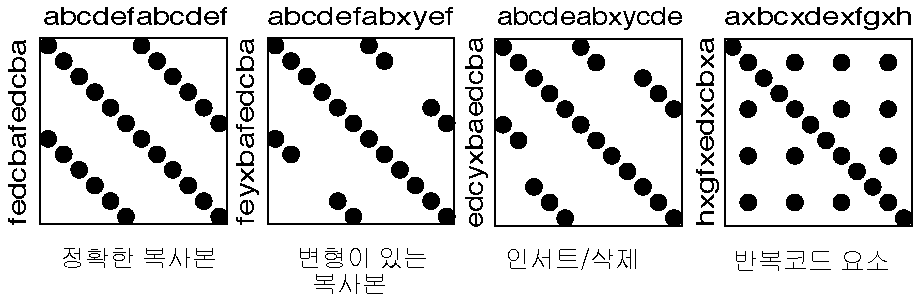
\includegraphics[width=\textwidth]{DuplicationDotplot}
\caption{Possible sequences of dot and their associated interpretations.}
\figlabel{DuplicationDotplot}
\end{center}
\end{figure}

Some interesting configurations formed by the dots in the matrices are the following:

\begin{bulletlist}
\item \emph{Exact Copies:} diagonals of dots indicate copied sequences of source code.

\item \emph{Copies With Variations:} sequences that have holes in them indicate that a portion of a copied sequences has been changed.

\item \emph{Inserts/Deletes:} broken sequences with parts shifted to the right or left indicate that a portion of code has been inserted or deleted.

\item \emph{Repetitive Code Elements:} rectangular configurations indicate periodic occurrences of the same code. An example is the break at the end of the individual cases of a C or C ++ switch statement, or recurring preprocessor commands like \lct{\#ifdef SOME CONDITION}.
\end{bulletlist}

\subsection*{Tradeoffs}

\subsubsection*{Pros}

\begin{bulletlist}
\item The approach is largely language-independent, since only the code normalization depends on the language syntax.

\item The approach works well when reverse engineering large amounts of unknown code, because the dotplots attract your eye to certain parts of the code to be studied more closely.

\item The idea is simple yet works surprisingly well. A simple version of the approach can be implemented by a good programmer using a appropriate tools in a couple of days. (One of our better students made a small dotplot browser in Delphi in two days.)
\end{bulletlist}

\subsubsection*{Cons}

\begin{bulletlist}
\item Dotplots only present pairwise comparisons. They do not necessarily help you identify all instances of duplicated elements in the entire software system. Although the approach can easily be extended to present multiple files across each axis, the comparisons are still only pairwise.
\end{bulletlist}

\subsubsection*{Difficulties}

\begin{bulletlist}
\item A naive implementation of a dotplot visualizer may not scale well to large systems. Tuning and optimizing the approach for large data sets can compromise the simplicity of the approach.

\begin{figure}[t]
\begin{center}
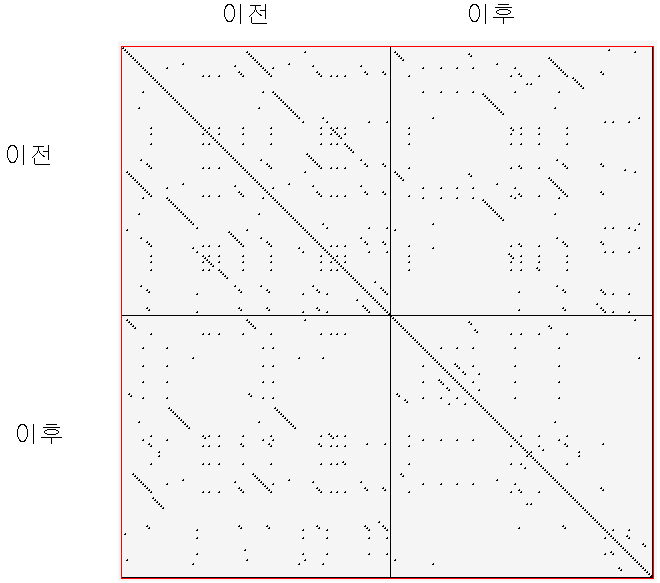
\includegraphics[width=0.8\textwidth]{DuplicationRefactoring}
\caption{Code duplication before and after refactoring.}
\figlabel{DuplicationRefactoring}
\end{center}
\end{figure}

\item The interpretation of the data may be more subtle than it appears at first glance. Indeed, while comparing multiple files the diagonals represent more duplication than is really in the system because we are comparing duplicated fragments with themselves over different files, as shown by \figref{DuplicationRefactoring} and \figref{DuplicationPython}.

\index{mural visualization}
\item The screen size limits the amount of information that can be visualized. Some success has been achieved with so-called ``mural'' visualization approaches \cite{Jerd96b}. However, these techniques are significantly more difficult to implement than simple dotplots and are not worth the extra effort.
\end{bulletlist}

\subsection*{Example}

In \figref{DuplicationRefactoring} we see a \ind{dotplot} of two versions of a piece of software, before and after the duplication has been removed. The first version is compared to itself in the top left square. The line down the diagonal simply shows us that every line of code is being compared to itself. What is more interesting is that several other diagonal lines occur in the dotplot, which means that code has been duplicated within this file. A second version of the same file is compared to itself in the lower right square. Here we see no significant duplication aside from the main diagonal, which reflects the fact that all the duplicated code has been successfully refactored.

\begin{figure}[h]
\begin{center}
\includegraphics[width=\textwidth]{DuplicationPython}
\caption{A Python file A being compared to itself and to a second file B.}
\figlabel{DuplicationPython}
\end{center}
\end{figure}

The bottom left and top right squares are mirror images of each other. They tell us how the before and after files have been reorganized. Since there is no strong diagonal, this tells us that significant reorganization has taken place. The diagonal stripes show us which parts of the old version have survived and where they appear in the new version. From the dotplot alone, we can guess that about half of the code has survived, and another half of the code has been significantly rewritten.

Dotplots are also useful to detect duplication across multiple files. \figref{DuplicationPython} shows a dotplot comparing two \ind{Python} files. The comparison of A vs. A shows that there is essentially no internal duplication. Very likely there are some switch statements in the bottom have of the file, indicated by the matrix pattern.

When we compare file A to file B, however, we detect a staggering amount of duplication. It looks very much like file B is just a copy of file A that has been extended in various ways. Closer investigation showed this to be the case. In fact, file A was just an older version of file B that had inadvertently been left in the release.

Dotplots can also be useful to detect other problems. \figref{DuplicationSwitch} presents four clones that represent a switch statement over a type variable that is used to call individual construction code. The duplicated code could perhaps be eliminated by applying \charef{Transform Conditionals to Polymorphism}{TransformConditionalsToPolymorphism}.

\begin{figure}
\begin{center}
\includegraphics[width=0.75\textwidth]{DuplicationSwitch}
\caption{Dotplots produced by four switch statements.}
\figlabel{DuplicationSwitch}
\end{center}
\end{figure}

\subsection*{Known Uses}

The pattern has been applied in biological research to detect DNA sequences \cite{Pust82a}. The Dotplot tool \cite{Helf95a} has been used to detect similarities in manual pages, literary texts and names from file systems. In the \ind{FAMOOS} project, the pattern has been applied to build \ind{Duploc}, a tool for identifying duplication in software source code \cite{Duca99b}. The \ind{Dup} tool \cite{Bake92a} has been used to investigated the source code of the X-Window system and uses a dotplot matrix graphical representation.

\subsection*{Related Patterns}

Once you have detected duplicated code, numerous refactoring patterns may apply, in particular \patpgref{Extract Method}{ExtractMethod}.

Very often duplicated code arises because clients assume too many responsibilities. In that case, \patpgref{Move Behavior Close to Data}{MoveBehaviorCloseToData} will help you to eliminate the duplication.

Dotplots also help to detect large conditional constructs. You should probably \charef{Transform Conditionals to Polymorphism}{TransformConditionalsToPolymorphism} to eliminate these conditionals and thereby achieve a more flexible design. 

%=============================================================
\ifx\wholebook\relax\else
   \bibliographystyle{alpha}
   \bibliography{scg}
   \end{document}
\fi
%=============================================================

